A diferencia de F0--F4, la política de \textit{hyperthreading}
(\texttt{smt\_policy}) sí se pudo medir directamente hoy: cambiarla no
requiere el permiso de escritura de frecuencia (P1/P4) que bloquea F0--F4,
porque \texttt{smt\_policy} solo determina qué IDs de CPU se declaran en
\texttt{cores.delegated\_cpus} -- una operación de afinidad
(\texttt{sched\_setaffinity()}) sin privilegios especiales, no una
escritura a \texttt{scaling\_governor} ni a MSRs de frecuencia.

\textbf{Diseño del barrido}: se fijaron los mismos 6 núcleos físicos de
\texttt{paccaA100} (0--5, confirmados vía \texttt{lscpu -e}) y se corrió
\texttt{npb\_cg} --- el kernel de referencia sugerido en el informe
anterior por su sensibilidad conocida a contención de caché --- bajo dos
configuraciones, 5 repeticiones cada una: (1) \texttt{delegated\_cpus=[0..5]},
\texttt{smt\_policy=one\_thread\_per\_physical\_core}, 6 hilos OMP, la
política vigente en producción; (2) \texttt{delegated\_cpus=[0,16,1,17,2,18,
3,19,4,20,5,21]} (ambos hermanos SMT reales de cada uno de los mismos 6
núcleos físicos), \texttt{smt\_policy=all\_threads}, 12 hilos OMP.

\begin{table}[H]
\centering
\caption{IPC medio, MPKI y tasa de fallos LLC, npb\_cg, 6 núcleos físicos fijos (5 repeticiones c/u).}
\label{tab:smt-policy}
\small
\begin{tabular}{@{}lrrrrr@{}}
\toprule
\textbf{Política} & \textbf{Hilos} & \textbf{IPC medio} & \textbf{CV\% IPC} & \textbf{MPKI} & \textbf{Tasa fallos LLC} \\
\midrule
\texttt{one\_thread\_per\_physical\_core} & 6  & 1{,}770 & 0{,}45\,\% & 20{,}80 & 0{,}865 \\
\texttt{all\_threads}                     & 12 & 1{,}055 & 0{,}44\,\% & 20{,}81 & 0{,}865 \\
\bottomrule
\end{tabular}
\end{table}

\begin{figure}[H]
\centering
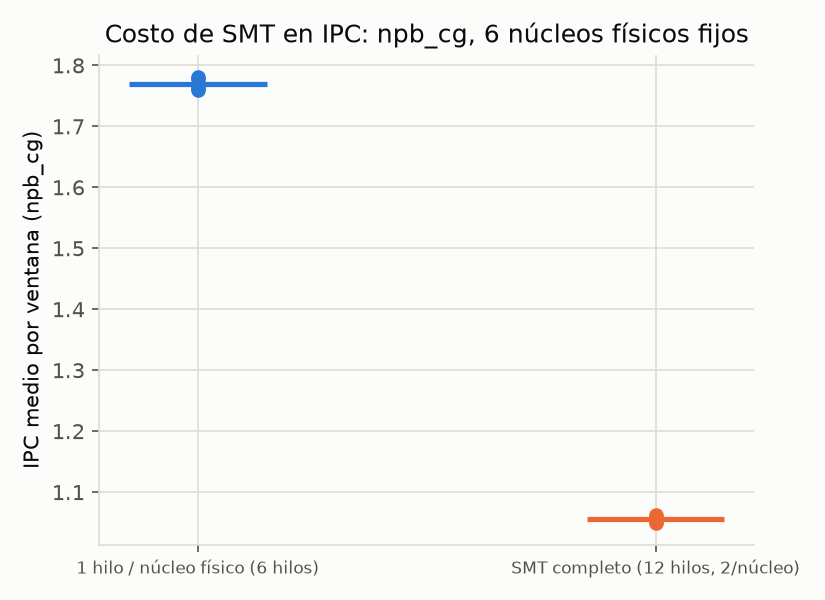
\includegraphics[width=0.75\textwidth]{../plots/smt_policy_ipc.png}
\caption{IPC por ventana, npb\_cg, 5 repeticiones por política (línea horizontal = media).}
\label{fig:smt-policy-ipc}
\end{figure}

\textbf{Resultado}: activar ambos hermanos SMT en los mismos 6 núcleos
físicos reduce el IPC medio de \texttt{npb\_cg} en 40{,}4\,\% (1{,}770 a
1{,}055), con una variabilidad intra-política casi idéntica y despreciable
en ambos casos (CV\%$<$0{,}5\,\% en las dos), es decir, el efecto es
sistemático y no ruido de medición. Notablemente, MPKI y la tasa de fallos
de LLC \textbf{no cambian} entre políticas (20{,}80 vs.\ 20{,}81 MPKI;
0{,}865 en ambas) -- eso descarta que la caída de IPC venga de más tráfico
de caché de último nivel.

\textbf{Límite real de este diseño experimental, que debe declararse}:
esta comparación cambia dos cosas a la vez, no solo la ocupación de SMT --
al pasar de 6 a 12 \texttt{delegated\_cpus}, \texttt{OMP\_NUM\_THREADS}
también pasa de 6 a 12, así que el paralelismo de OpenMP de \texttt{npb\_cg}
cambia junto con la política de SMT. Que MPKI y la tasa de fallos de LLC
se mantengan estables es evidencia compatible con "contención de
\textit{pipeline} entre hermanos SMT" -- el mecanismo que
\texttt{one\_thread\_per\_physical\_core} fue diseñado para evitar -- pero
no la aísla de otras causas posibles del mismo efecto: ancho de banda de
memoria compartido entre los 12 hilos, latencia de sincronización de
OpenMP con el doble de hilos, contención de front-end, o presión sobre las
unidades de carga/almacenamiento. Un diseño que aislara la causa exacta
requeriría mantener \texttt{OMP\_NUM\_THREADS} fijo en 6 y solo cambiar a
qué IDs de CPU se pinan (por ejemplo, 6 hilos sobre 6 núcleos físicos vs.\
6 hilos sobre 3 núcleos físicos con SMT, 2 por núcleo) -- una extensión
concreta no realizada aquí. Lo que sí queda establecido con esta medición,
sin ambigüedad, es que la caída de IPC es real y sistemática bajo SMT
completo, no que su causa exacta sea única y exclusivamente contención de
\textit{pipeline}.

El tiempo total de pared fue, además, \textbf{menor} bajo
\texttt{all\_threads} (5{,}76\,s vs.\ 6{,}82\,s) -- el doble de hilos
completa el trabajo fijo de \texttt{npb\_cg} más rápido pese al IPC por
hilo más bajo. Como el proyecto optimiza EDP (energía $\times$ tiempo), no
tiempo por sí solo, este resultado \textbf{no permite concluir} que
\texttt{one\_thread\_per\_physical\_core} sea la configuración
energéticamente superior -- no se midió energía en este barrido. Su
justificación aquí es distinta y más limitada: aislar la medición de
telemetría/IPC de Fase 1 de un sesgo de contención conocido, no una
afirmación sobre eficiencia energética.

\textbf{Conclusión (con el alcance correcto)}: \texttt{smt\_policy=one\_thread\_per\_physical\_core}
queda confirmado con medición directa como la política que evita un sesgo
sistemático y grande (40{,}4\,\%) en el IPC medido, con evidencia compatible
con -- pero no exclusivamente demostrativa de -- contención de recursos de
\textit{pipeline} entre hermanos SMT como mecanismo. No debe leerse como
una confirmación de que esta política sea la energéticamente óptima para
Fase 4; esa es una pregunta distinta, no respondida aquí.
